\chapter{Classification}
Classification is the final step for object detection in satellite images. Based on the extracted features from the images we classify them using some standard classifier, e.g, support vector machines (SVM), MLP etc. The classifier learns the patterns from the features of an image and predicts the label of that image.

\section{Support Vector Machine (SVM)}
SVM \cite{b3} is used to classify two classes by finding the best hyper-plane between those two classes. The data points that are closest to the hyper-plane from the two classes are called support vectors. SVM maximizes the distance between the support vectors belonging from two different classes. The equation of the hyper-plane can be written as: 
$$\vec{w}\cdot \vec{u}+b=0$$ where $\vec{w}$ and $b$ are the weight vector and bias respectively. $\vec{w}$ is perpendicular to the hyper-plane. Now, the decision rule for SVM can be defined as:
$$\vec{w}\cdot \vec{u}+b\geq +1,\ then\ positive\ class$$ , $$\vec{w}\cdot \vec{u}+b\leq -1,\ then\ negative\ class$$
Support vectors from positive and negative class will satisfy the equation \ref{eq1} and \ref{eq2} respectively.
\begin{equation}
    \vec{w}\cdot \vec{u}+b=+1
    \label{eq1}
\end{equation}
\begin{equation}
    \vec{w}\cdot \vec{u}+b=-1
    \label{eq2}
\end{equation}
One example of SVM is given in figure \ref{fig13}.

\begin{figure}[!htbp]
\centerline{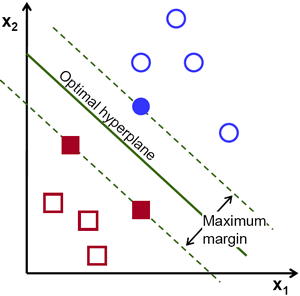
\includegraphics[height=60mm,width=60mm]{img/fig13.png}}
\caption{Working of SVM. Source:https://docs.opencv.org/}
\label{fig13}
\end{figure}

Now, we can find out the distance between support vectors from two class and maximize that distance with respect to $\vec{w}$ and $b$. 

\par The authors of \cite{b6} has used linear SVM to classify between oil-tank and non oil-tank images. The features were extracted using HOG and CNN. These feature vectors will be represented as data points as described above. 


\section{Multi-layer Perceptron (MLP)}
\par Chen et.al. \cite{b8} and Wu et.al. \cite{b5} has used MLP for classification. Multi-layer perceptron is a classifier based on the concept of artificial neural networks. It has feed-forward architecture, where the input is propagated through each computational layer. MLP has atleast three layers:
\begin{itemize}
    \item \textbf{Input layer: } In this layer we provide the extracted feature as input through various neurons. If a feature vector has 10 components then the input layer will have 10 neurons. In each neuron we will feed one component of the feature vector as input.
    \item \textbf{Hidden layer: }There could be many hidden layers in a MLP. A hidden layer can have any number of nodes. In each node, outputs of all the neurons from previous layer will be multiplied with a weight vector and then a bias will be added to it. The result of this operation will be passed to a non-linear activation function which will produce either 0 or 1. This whole operation happen in each node of the hidden layer.
    \item \textbf{Output layer: }The number of nodes in this layer depends on the type of classification. If we are doing binary classification then there will be only one node. In this node the same operation will happen as that of the hidden layer node. And it will output the label of the input as either 0 or 1. 
\end{itemize}
The structure of a multi-layer perceptron is given in figure \ref{fig14}.

\begin{figure}[!htbp]
\centerline{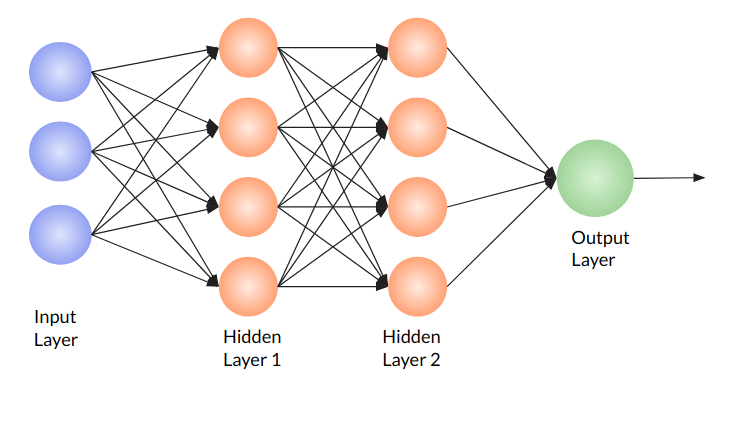
\includegraphics[height=60mm,width=110mm]{img/fig14.png}}
\caption{Architecture of MLP}
\label{fig14}
\end{figure}

\par MLP works using two algorithms:
\begin{itemize}
    \item \textbf{Forward propagation: }Here, we introduce weights and bias in each hidden layer. The computation in each node will be given as: 
    $$y_i=\sum_{n=1}^{K}w_i\cdot x_i+b,\ and$$
    $$z_i=g(y_i)$$
    where $g$ is the non-linear activation function. This function outputs value within 0 and 1 or within -1 and +1, e.g, \textit{sigmoid} function outputs in the range 0 and 1, while \textit{tanh} function outputs in the range of -1 to +1.
    \par This process will continue until the output layer is reached, which will output a label, i.e, either 0 or 1. Based on the predicted value we calculate the loss using any loss function, e.g, cross-entropy loss. We give all the images and get an output label for each of the images along with their loss. The summation of all the loss function is known as cost function. In backpropagation algorithm we minimize this cost function.
    \item \textbf{Backward propagation: }Here, we differentiate the cost function w.r.t weight vector and bias of the previous layer and we update its weight and bias by using the formula: $w_i=w_i-\Delta w_i$ and $b_i=b_i-\Delta b_i$. We keep on updating the weights in each layer and move backwards. When we reach the input layer, we again perform the forward propagation with the updated weights. 
\end{itemize}



